\documentclass[modern]{aastex631}
\usepackage{hyperref}
\bibliographystyle{aasjournal}
\turnoffedit
\usepackage[caption=false]{subfig}
\usepackage{booktabs}
\usepackage{censor}
\usepackage{mathtools}
\usepackage{outlines}
\usepackage{amsmath,bm}

\def\Teff{T_{\rm eff}}
\def\vsini{v\sin{i}}
\def\kmps{\mathrm{km}\;\mathrm{s}^{-1}}

\begin{document}
\shorttitle{blas\'e}
\shortauthors{Gully-Santiago}
\title{Transfer learning for \'echelle spectroscopy with \texttt{blas\'e}}

\author{Michael Gully-Santiago}
\affiliation{University of Texas at Austin Department of Astronomy}

\author{Caroline V. Morley}
\affiliation{University of Texas at Austin Department of Astronomy}

\begin{abstract}

 We introduce blas\'e, a framework for transfer learning for high-grasp echelle spectroscopy.  \texttt{blas\'e} produces extensible models that are both physically informed and highly accurate when compared to data. These models can be evaluated quickly for use in likelihood calculations. It works on data with large spectral grasp: simultaneously wide bandwidth and high spectral resolution.


\end{abstract}

\keywords{High resolution spectroscopy (2096), Stellar spectral lines (1630), Astronomy data modeling(1859), GPU Computing (1969), Calibration (2179), Radial Velocity (1332), Maximum likelihood estimation (1901), Deconvolution (1910), Atomic spectroscopy (2099), Stellar photospheres (1237)}, 

\section{Introduction}\label{sec:intro}

\subsection{Spectral fitting past and present}

Tens of thousands or more individual spectral lines give rise to a sea of undulations that imbue each stellar spectrum with its characteristic appearance.  The identification and understanding of these lines has defined a large category of astrophysics over the last century.  The field grew from by-eye catalogs of stellar templates \citep{1901AnHar..28..129C} to quantifying the role of atomic ionization balance \citep{1925PhDT.........1P}, to modern synthetic forward models including millions or billions of lines \citep{husser13, 2021ApJ...920...85M}.  As technology has improved, our data and models have become more voluminous, more precise, and more complicated.  The mere act of comparing models to observed spectra can resemble a computational statistics challenge as much as a scientific one.  Here we introduce a machine-learning-based framework \texttt{blas\'e} aimed at solving computational, statistical, and scientific challenges associated with data-model comparisons for modern astronomical spectroscopy.

The metaphorical holy grail of astronomical spectroscopy is a function that takes in an observed astronomical spectrum and reports back the postition, amplitude, width, and shape of all of its spectral lines, automatically, accurately, and precisely.  The function would go further, to report back the systemic radial velocity (RV) and rotational broadening ($v\sin{i}$).  Finally the function would---in an \emph{Inception}-like manner---provide what it believes to be the interpretable generating function that produced the data, so that we may gain insights on future examples of this or other stars.  Solving this problem is hard, for at least four reasons.  First, the spectral lines may overlap, and so the assignment of one line may be partially degenerate with the assignment of some other adjacent line.  Second, extremely wide line wings blend into the continuum, such that the placement of the continuum level may become ill-defined.  Third, the extent of line blending and realized line shape depends strongly on the spectral resolution of the spectrograph, the rotational broadening of the star, and possibly the instrumental configuration at the time of observation.  Finally, telluric absorption lines commingle with the astronomical spectral lines of interest, censoring some spectral regions entirely, or partially confounding other lines with chance allignments.

Addressing these and other challenges forms the backbone of \emph{spectral calibration}, an increasingly valuable specialty as the deficits in our models become intolerable with greater data quantity and quality.  Luckily, many scientific applications in astrophysics do not need the technically demanding noise-free template, nor catalog-of-all-spectral-lines.  A few lines suffice.  For those applications, human inspection of isolated lines and semi-automated equivalent width determination have been and will remain adequate.  

But many new and important questions in the fields of stars and exoplanets aspire to reach the margins of what the entire dataset can inform.  In particular, data from high-\emph{grasp} \'echelle spectrographs possess simultaneously high spectral resolving power and high bandwidth, yielding tens of thousands or possibly millions of independent spectral resolution elements for each star, substar, or exoplanet.  Those applications that seek to gain signal by ``stacking'' spectral lines or cross-correlating templates can hypothetically gain huge boosts in the accessible signal-to-noise ratio compared to a single or few lines.  Most manual and semi-automated methods cannot take advantage of the entire spectral bandwidth, or rely on exact knowledge of the underlying templates and may fail to achieve the hypothetical promise of these high-bandwidth spectrographs \citep{2020AJ....160..198H}.

For example, exoplanet cross-correlation spectroscopy \citep{2013MNRAS.436L..35B} hinges on accurate molecular spectral templates to detect and characterize the atmospheres of exoplanets.  Imperfections in these templates can mute the perceived signal strength of these atmospheric features \citep{2015A&A...575A..20H}.  
In extreme precision radial velocity (EPRV) applications, cross-correlation methods work, but addressing telluric absorption at the $\mathrm{cm/s}$ level may require joint modeling of the star and the Earth's atmospheric absorption before convolution with an instrumental kernel \authorcomment1{speakerdeck.com/dwhgg/telluric-line-hack-week-wrap-up}).

In the case of Doppler imaging, an accurate underlying template is needed to detect longitudinally symmetric structures such as polar spots \citep{1983PASP...95..565V, roettenbacher16} or zonal bands \citep{Crossfield14,2021ApJ...906...64A}.  

Existing open-source frameworks have overcome some of these challenges, or have been purpose-built for specialized applications. 
These frameworks include \texttt{ROBOSPECT} \citep{2013PASP..125.1164W}, \texttt{specmatch} \citep{2015PhDT........82P}, \texttt{specmatch-emp} \citep{2017ApJ...836...77Y}, \texttt{wobble} \citep{2019AJ....158..164B}, \texttt{starfish} \citep{czekala15}, \texttt{sick} \citep{2016ApJS..223....8C}, \texttt{psoap} \citep{2017ApJ...840...49C}, \texttt{FAL} \authorcomment1{Cargile et al. in prep}, CHIMERA \citep{2015ApJ...807..183L}, the \texttt{Cannon} \citep{2017ApJ...836....5H},  \texttt{MINESweeper} \citep{2020ApJ...900...28C}, and recently \texttt{ExoJAX} \citep{2022ApJS..258...31K}.  
The design of these frameworks necessarily have to make a choice in the bias-variance tradeoff: is the tool more \emph{data}-driven or more \emph{model}-driven?  The statistical tradeoff can be viewed as a concession in physical self-consistency for model flexibility: more or fewer parameters.

A key new enabling technology breaks the historic limits of data-model comparisons for astronomical spectroscopy.  Automatic differentiation \citep[``autodiff'',][]{2015arXiv150205767G} and the backpropagation algorithm has revolutionized machine learning and neural network architecture design, and is increasingly applied in astrophysical data analysis contexts, \emph{e.g.} kernel phase coronography with \texttt{poppy} \citep{2021ApJ...907...40P}, and exoplanet orbit fitting with \texttt{exoplanet} \citep{2021JOSS....6.3285F}.  Of the spectroscopy frameworks mentioned above, \texttt{wobble} \citep{2019AJ....158..164B} and \texttt{ExoJAX} \citep{2022ApJS..258...31K} employ autodiff technology.  \texttt{wobble} treats each pixel as a tunable control point, producing $\sim10^5$ parameters for a modern stellar spectrum.  The \texttt{ExoJAX} framework has only $\sim$dozens of tunable parameters that describe the fundamental physical properties controlling a brown dwarf atmosphere.  These two autodiff-aware frameworks span the extreme ends of non-parametric and parametric modeling for spectroscopy.

In this paper we show that autodiff-aware semi-empirical models offer a cozy middle ground: informed from self-consistent models, but refined with data.  In Section \ref{methodology} we show how to supplant the computationally expensive radiative transfer, by cloning pre-computed synthetic spectral models.  In Section \censor{XX} we describe how to fine-adjust the cloned models to data in a transfer-learning step.  Section \censor{XX} exhibits some injection-recovery type tests on simulated data of known properties.  In Section \censor{XX} we show real-world data from high-grasp near-IR spectrographs.  Finally we discuss many conceivable extensions to the framework, and directions for future work in Section \censor{xx}.


\section{Methodology}\label{methodology}

\subsection{Overall Architecture and Design Choices}

We start with a high resolution pre-computed synthetic stellar model spectrum, $\mathsf{S}(\bm{\lambda})$. The procedure is largely agnostic to the exact details of how this spectrum was made. For the purposes of this paper, we will showcase examples from two well-known families of precomputed synthetic spectra: \texttt{PHOENIX} \citep{husser13} for stellar spectra $(T_{\mathrm{eff}}\in [2300, 10000]\;K)$ and \texttt{Sonora} \citep{2021ApJ...920...85M} for brown dwarf spectra $(T_{\mathrm{eff}}\in [1000, 2300]\;K)$. We place the following demands on the precomputed spectra. They should have sporadic regions of discernable continuum devoid of lines, and the continuum must vary smoothly in wavelength. The spectral lines or pseudo-lines should be resolved, and not sub-sampled. We suspect most stellar spectra meet these criteria, except for the coolest M dwarfs and brown dwarfs. The method can hypothetically handle spectra without discernable continua, but we suspect some modifications to the preprocessing steps would be needed. We truncate the red and blue limits of the precomputed synthetic spectrum to match a high-bandwidth echelle spectrograph, extended with a buffer at the edges of size $\pm \Delta \lambda_{\mathrm{buffer}}$, chosen to account for plausible radial velocity and rotational broadening of real stars. A generous buffer of $v \sin{i} < 500 \;\kmps$ and $|RV|<500 \;\kmps$ yields a typical buffer of about 30~\AA.

The choice of limiting the bandwidth to a region-of-interest around a single echelle spectrograph bandwidth stems from computational constraints. In principle, there is no fundamental limit to the bandwidth one could clone with the method presented here, up to and including the entire precomputed synthetic spectral model bandwidth. We adopt the exact native wavelength sampling with no smoothing or interpolation, yielding a wavelength vector $\bm{\lambda}_s$ with length $N_\mathrm{s}$ equal to the number of pixels within the extents of our region of interest including the buffers.

At this stage, we have the choice of whether to work in linear or log scale flux units. Adopting the log of the flux would ensure that the cloned model possesses only positive flux values, a desirable trait of any physical spectral model. We chose instead to stick with native linear flux scaling because of the availability of convenient approximations to astrophysically relevant line profiles in the linear scaling domain. We normalize the spectrum by its median value since we do not intend to apply these methods to absolutely flux calibrated spectra.

\subsection{Initialization}

We initialize the cloned model with a series of preprocessing steps. We divide the entire spectrum by a black body of the same effective temperature $T_{\mathrm{eff}}$ as the model template. The resulting signal typically possesses a smooth continuum variation. An additional continuum flattening step ensures that subsequent spectral line finding steps get applied uniformly. Here, we identify the continuum regions by the most prominent peaks in the specturm separated by a distance of at least 5,000$-$90,000 pixels from adjacent peaks, yielding between 60 and 5 control points. We then fit an $n_{\mathrm{poly}} = 3^{rd}-15^{th}$ order polynomial to these peaks, evaluate the polynomial on the entire bandwidth $\mathsf{P}(\bm{\lambda}_s)$, and divide the spectrum by this trend. Visual inspection of this continuum-flattened spectrum typically possesses variations at the $<1\%$ level. Tuning the pixel distance and polynomial order can lower the undulations to $<0.05\%$ level for some input spectra. We found a pixel distance of 50,000 and $3^{rd}$ order polynomial worked across the range of effective temperatures for HPF's bandwidth. The IGRINS spectra had more significant continuum opacity and band heads to accommodate and therefore needed to capture finer-scale variation: 5,000 pixels and a $9^{th}$ order polynomial appeared adequate over most of the effective temperature range.

This high-pass filtering step should be set to capture the genuine spectral shape, without over-fitting broad line-wings such as those in deep Hydrogen and sodium lines. We have experimentally found it helpful to hand-tune models of exceptionally broad and non-standard line wings with an optional pre-processing step that depends on the wavelength range of interest. Here we sketch the approach for common broad lines found in the long-wavelength visible and near-infrared wavelength regions.

% TODO We pre-assign spectral lines for the conspicuous Hydrogen lines and neutral metal lines. Table

We emphasize that a recreation of the unvarnished input spectrum can be obtained by multiplying the continuum-flattened signal by the ``perturbed black body'', $\mathsf{B}(\bm{\lambda}_s)\cdot \mathsf{P}(\bm{\lambda}_s)$, that symbolizes the black body modulated by continuum opacity or broad-band radiative transfer effects. This smooth spectrum may be useful for applications that need to keep track of broad-band flux, such as low-resolution spectra, or regions with molecular band heads. The ``perturbed black body'' continuum model contains $n_{\mathrm{poly}}+1$ fixed-but-possibly tunable lookup parameters, plus the fixed input $T_{\mathrm{eff}}$.

Next, we identify the spectral lines. We apply a local-minimum-finding algorithm on the spectrum by defining a prominence threshold $P_{rom} \in (0.005, 0.02)$. This threshold dictates the number of lines that will be modeled: a lower prominence finds more, weaker lines, and a larger prominence finds fewer, deeper lines. The prominence algorithm successfully finds lines that reside on top of broad line wings, or unresolved band heads provided that the individual lines exceed the prominence threshold in their local region. The number of lines $N_{\mathrm{lines}}$ depends on the bandwidth, prominence, and the intrinsic properties of the input spectrum, principally effective temperature and metallicity.

For this paper, we illustrate examples for two \'echelle spectrographs with particularly large spectral grasp: the Habitable Zone Planet Finder \citep[HPF,][]{2014SPIE.9147E..1GM} on the Hobby-Eberly Telescope at McDonald Observatory in Fort Davis, Texas; and the Immersion Grating Infrared Spectrograph \citep[IGRINS,][]{park14}
currently on the Gemini South Telescope on Cerro Pach\'on in Chile. The $R=55,000$ HPF has a native bandwidth of $8079-12785$~\AA, which we expand to $8049-12815$~\AA~including the edge buffers. IGRINS has two cameras for $H$ and $K$ band, with the combined spectrum spanning $14267-25217\;$\AA~ including the edge buffers and the region in-between the two cameras, all at a resolving power of $(R=45,000)$. The spectrograph acquisition, reduction, and post-processing steps yield data $\mathsf{D}(\bm{\lambda}_{d})$, where $\bm{\lambda}_{d}$ is the wavelength vector at the instrumental resolution and sampling of each instrument, generally much coarser than the resolution and sampling grid of the precomputed synthetic spectra. The data wavelength vector may also contain gaps between \'echelle orders, whereas the precomputed wavelength coordinates are usually contiguous. HPF may have up to $2048\times28=$57,344 pixels, and IGRINS has typically about 75,000 pixels, after common trimming of noisy edge pixels and unusable telluric regions.


\begin{figure}[hbt!]
 \centering
 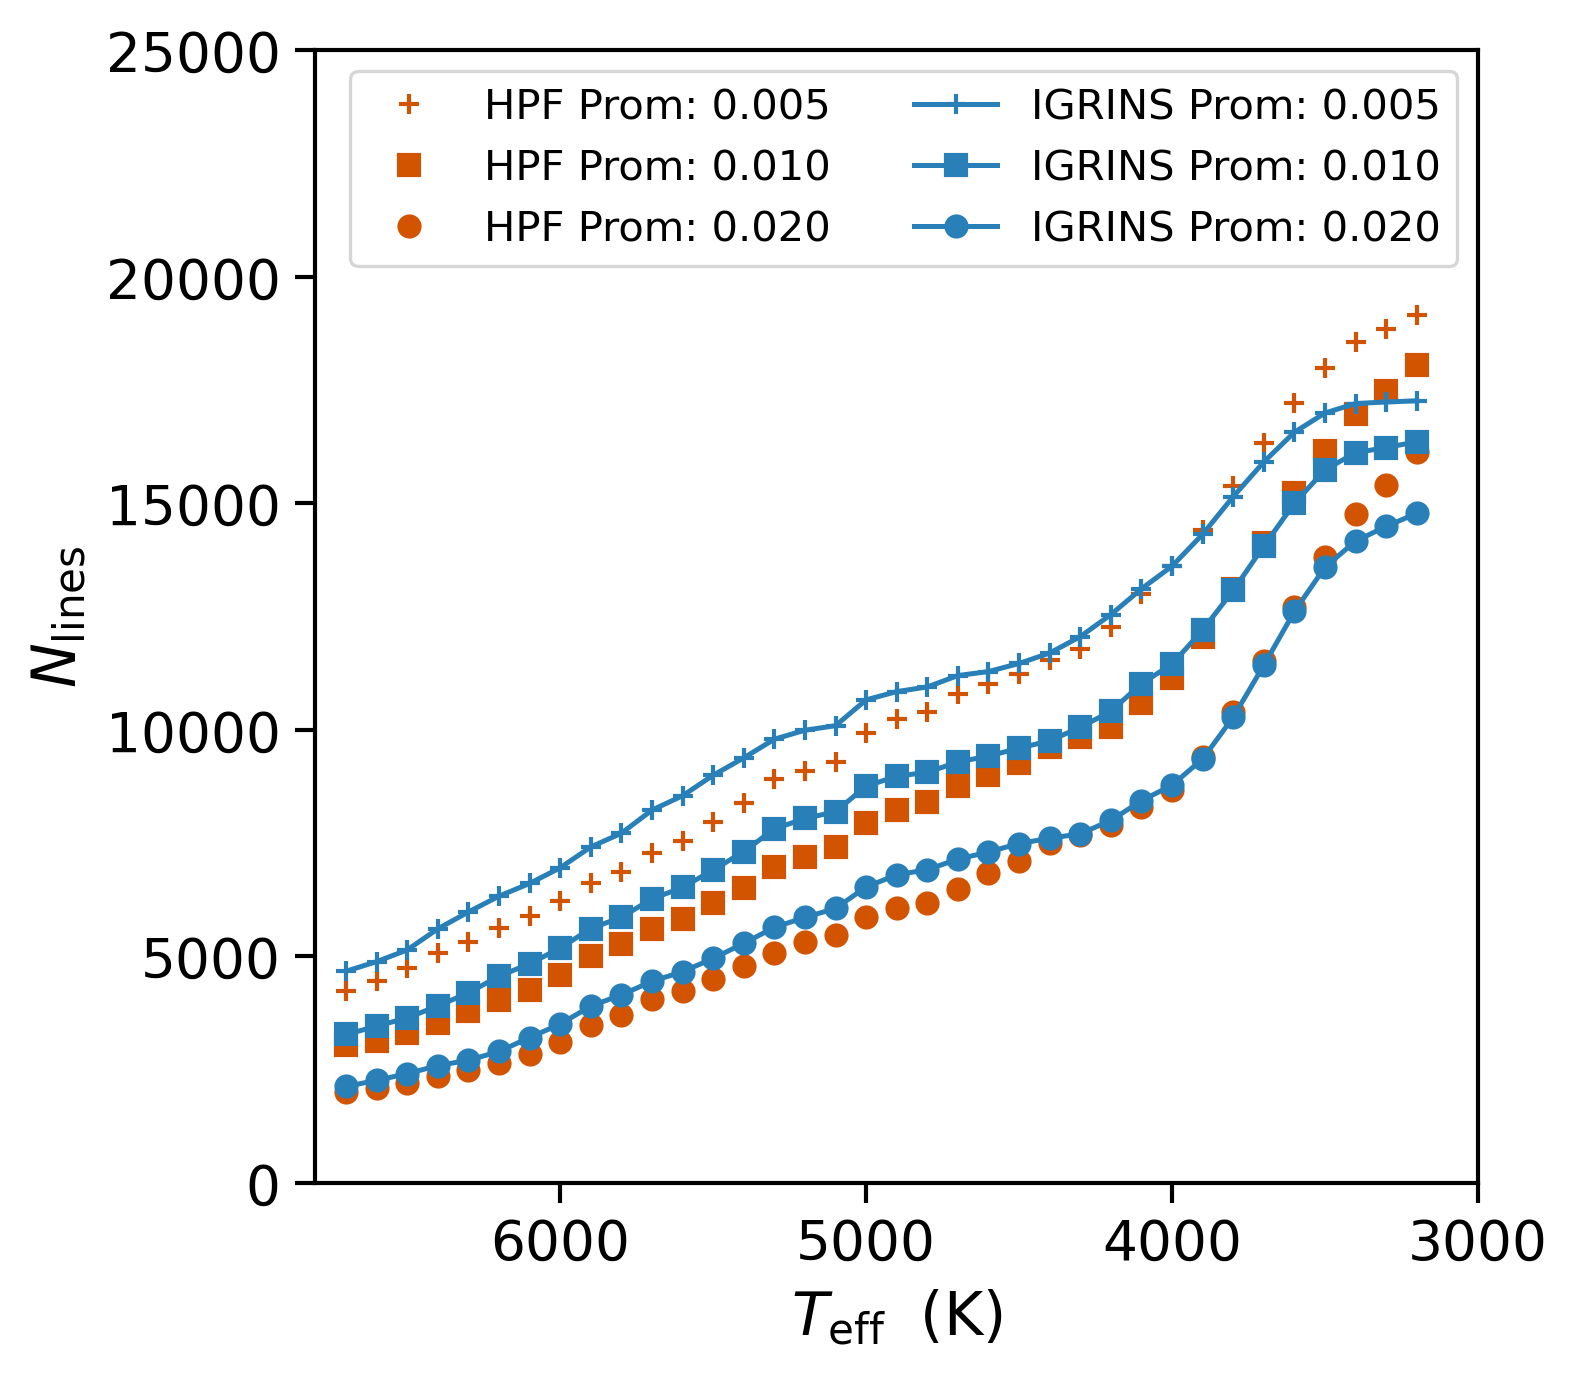
\includegraphics[width=0.5\textwidth]{figures/N_lines_vs_Teff_prom.png}
 \caption{Number of prominent spectral lines versus effective temperature for PHOENIX models truncated to IGRINS (\emph{blue, connected} points) and HPF (\emph{orange, free-standing} points) bandwidths, for different prominence thresholds of $0.02$, $0.01$, and $0.005$.}
 \label{fig_Nlines_vs_teff}
\end{figure}


Figure \ref{fig_Nlines_vs_teff} shows how the number of detected lines $N_{\mathrm{lines}}$ scales with effective temperature and prominence threshold $P_{rom}$ for the \texttt{PHOENIX} grid, truncated to the bandwidths-plus-buffers for HPF and IGRINS. We see between about 2,000 and 20,000 lines depending on the $T_{\mathrm{eff}}$ and $P_{rom}$. HPF and IGRINS have a comparable number of lines, and halving the prominence increases the number of lines by about $20-30\%$ in these ranges. The number of lines monotonically increases towards cooler effective temperatures.
The HPF-truncated spectra have $N_s=$335,849 native resolution samples, comparable to the IGRINS-truncated spectra, $N_s=$330,052.

So far we have only one piece of information about the peaks: their location. Next, we derive coarse properties about each detected peak: its amplitude and width, again using the prominence algorithms implemented in \texttt{scipy} \citep{2020SciPy-NMeth}.

There does not exist a general-purpose, single-shot algorithm for obtaining the lineshape in the presence of overlapping spectral lines: where do the wings of one line begin and the wings of another adjacent line end? We, therefore, do not attempt to determine anything about the lineshape at this stage and instead assume that the lines resemble a Voigt profile, with a guess width about equally split between Lorentzian and Gaussian.

\subsection{The \emph{blas\'e} clone model}

We have now arrived at the \emph{blas\'e} clone model $\mathsf{M}(\bf{\lambda}_s)$ for a flattened synthetic spectrum $\mathsf{S}$: it is the cumulative product of transmission through the sea of all overlapping spectral lines:

\begin{eqnarray}
 \mathsf{M}(\bm{\lambda}_s) = {\displaystyle \mathsf{P} \prod_{j=1}^{N_{\mathrm{lines}}} (1-a_j \mathsf{V}(\bm{\lambda}_s-\lambda_{c,j}, \sigma_j, \gamma_j) )} \label{equation1}
\end{eqnarray}

where $\mathsf{V}(\lambda, \sigma_j, \gamma_j)$ is the normalized Voigt profile with Gaussian standard deviation $\sigma$, Lorentzian half-width $\gamma$, at line center position $\lambda_c$, for the $j^{th}$ spectral line. The amplitude $a$ is always expected to be positive for absorption lines and is equal to the area under the curve of the line since the Voigt profile is normalized. The optional Prefactor term $\mathsf{P}$ is fixed at $1$ by default but can be allowed to vary to fine-adjust imperfections leftover from the polynomial-based continuum flattening procedure.

\subsection{Voigt profile evaluation}
The Voigt profile $\mathsf{V}(\lambda, \sigma_j, \gamma_j)$ can be computed in exact closed-form using the Fadeeva function\authorcomment1{citation}. Evaluation of the Fadeeva function can be computationally costly, and so approximate forms may be desirable. Here we adopt the pseudo-Voigt approximation described in \censor{some paper}\authorcomment1{look up reference to PseudoVoigt}.

Two sampled Voigt approaches could be feasible. Direct convolution of a sampled Gaussian and Lorentzian profile may be too costly and inexact if pixels are coarsely sampled. Analogously, the convolution can be achieved in the Fourier domain through the multiplication of the Fast Fourier Transforms of the Gaussian and Lorentzian profiles, followed by the subsequent Inverse Fourier Transforms. The main rationale for either of these two choices would be to anticipate and align with planned convolutions such as rotational broadening and instrumental kernels. We do not currently implement these sampled convolutions in \emph{blas\'e} due to their prohibitive computational cost.


\subsection{Goodness of fit metric}
The model evaluated with its coarse initial values would have terrible performance: it would only vaguely resemble the synthetic spectral model, with up to $\pm 50\%$ undulations from the inexact assignment of widths, lineshapes, and amplitudes. Instead, we tune the parameters of the model, starting from these coarse initial values. This model has $N_{\mathrm{lines}}\times 3$ free parameters, where the center wavelength is held fixed and the amplitude, width, and lineshape are allowed to vary. We minimize a scalar ``goodness-of-fit'' metric, \emph{aka} loss scalar $\mathcal{L}$, chosen as the mean squared error (MSE), which is proportional to $\chi^2$, the sum of the squares of the residual vector $\mathsf{R} \equiv \mathsf{S}-\mathsf{M}$ but has no notion of per-pixel noise since the precomputed synthetic spectrum has no uncertainty:

\begin{eqnarray}
 \mathcal{L} = \sum_i^{N_s} (S_i - M_i)^2 = \mathsf{R^\intercal}\cdot \mathsf{R}
\end{eqnarray}


As seen in Figure \ref{fig_Nlines_vs_teff}, the number of lines can exceed 7,000, meaning the model has over 7,000 $\times 3 =$ 21,000 free parameters. Fitting that large number of parameters is difficult with conventional optimizers, which struggle to converge after hundreds of parameters\authorcomment1{Citation to limits of optimizers}.

Here we employ a variant of Stochastic Gradient Descent (SGD), an optimization technique that can scale to a virtually unlimited number of parameters\authorcomment1{provide a citation}. This technique computes the derivative of the loss scalar with respect to each of the parameters, the Jacobian: $(\frac{\partial \mathcal{L}}{\partial a_j}, \frac{\partial \mathcal{L}}{\partial \sigma_j}, \frac{\partial \mathcal{L}}{\partial \gamma_j})$. The Jacobian indicates how the MSE would decrease with a change in the parameter-of-interest, or put simply which-way and by-how-much you have to change the line properties to get a better fit.

The optimizer updates the $a_j, \sigma_j, \gamma_j$ parameters by a small fraction of the Jacobian---called the learning rate LR---towards the direction that would improve the fit, for all $N_{\mathrm{lines}} \times 3$ parameters simultaneously. The Jacobian is calculated behind the scenes with automatic differentiation\authorcomment1{Citation} implemented as the so-called backpropagation algorithm or simply ``backprop''. We choose the \texttt{PyTorch} framework that computes these Jacobians efficiently for all of the mathematical primitives in our \texttt{blas\'e} implementation.

In principle, we could compute the Jacobians analytically---since the partial derivatives of the Voigt function are known in closed-form---circumventing the vendor lock-in and memory overhead of an autodiff implementation with PyTorch. Further, an autodiff-aware implementation of the \emph{celerit\'e} algorithm\authorcomment1{add DFM citation} does not yet exist in PyTorch, constricting our choices for simultaneous continuum fitting. In practice, PyTorch also offers hardware acceleration (on GPU or TPU)\authorcomment1{citation needed}, mature support for a range of optimizers, and other perks that motivated its choice over analytic implementations or other machine learning frameworks. The GPyTorch framework\authorcomment1{add citation} may offer a workaround to the absence of a \emph{celerit\'e} implementation. Still, the performance of an analytic Jacobian implementation over the autodiff route presented here offers an interesting avenue of future research.

\subsection{GPU and Autodiff specific considerations}
We make a few tweaks to the implementation for numerical purposes. First, we want all the parameters to be positive, forbidding negative amplitudes and negative widths. We, therefore, tune the natural log of the parameters and exponentiate them before inclusion in Equation \ref{equation1}. Second, we found through iterative experimentation that the initialization amplitudes and widths were systematically shifted from the optimized values. We built-in scalar tweaks to the initialization amplitudes, Gaussian width, and Lorentzian width, which dramatically accelerated the optimization step.

We set the \texttt{requires\_grad=True} property for any Torch tensor that we want to vary. This allows us to easily explore whether, say, allowing the $\lambda_c$ parameter to vary significantly improves the fit. It also allows us to tune or freeze an experimental wavelength-dependent pre-factor to Equation \ref{equation1} to correct for lingering imperfections in the otherwise-fixed continuum flattening procedure.

The computational bottleneck occurs at the evaluation of Equation \ref{equation1}, which includes the assembly of a $N_{\mathrm{lines}}\times N_{s}$ matrix $\bm{\bar{V}}$ assembled by stacking each Voigt profile $\mathsf{V}_j(\bm{\lambda}_s)$ on top of each other:

\begin{equation}
 \begin{pmatrix}
 \mathsf{V}_1(\bm{\lambda}_s) & \\
 \mathsf{V}_2(\bm{\lambda}_s) & \\
 \vdots & \\
 \mathsf{V}_{N_{\mathrm{lines}}}(\bm{\lambda}_s) &
 \end{pmatrix}
\end{equation}

Equation \ref{equation1} performs a type of tensor contraction, turning a $N_{\mathrm{lines}}\times N_{s}$ matrix into a $1\times N_{s}$ vector. The number of Floating Point Operations (FLOPS) scales with the number of entries in this matrix, with a scalar prefactor for the cost of evaluating a single line profile at a single wavelength point. Efficient GPU algorithms exist for tensor contractions such as this product along an axis of a matrix, allowing this computation to proceed quickly on modern machines\authorcomment1{add citation?}. In particular, the proprietary CUDA architecture for NVIDIA\textsuperscript{\tiny\textregistered} GPUs contains Tensor cores with specialized matrix math, although the algorithms place restrictions on floating precision depending on the particular hardware and software available. The chief bottleneck occurs when the storage of the $\bm{\bar{V}}$ matrix exceeds the available RAM of a GPU or CPU: the computation will fail with an ``Out of Memory'' exception. Modern NVIDIA GPUs have $8-40$ GB of RAM. The memory bottleneck is even more pernicious than mere storage of the $\bm{\bar{V}}$ matrix since the CPU/GPU also has to store the computation graph for autodiff. The computation graph takes up more memory than the matrix itself, so it is generally not possible to evaluate Equation \ref{equation1} in its entirety in one-fell-swoop. A remedy is needed.

\subsection{Minibatches}

Minibatches offer a natural solution to the line-by-line computational bottleneck while also providing optimization performance improvements. Minibatches act as a form of regularization, the principal source of stochasticity in the Stochastic Gradient Descent algorithm, which tends to have better convergence than full-batch Gradient Descent\authorcomment1{citation}. The Machine Learning/Artificial Intelligence (ML/AI) community employs minibatches to handle similar situations, in which the dataset volume exceeds the available GPU RAM. Our configuration departs slightly from the typical ML/AI situation since their models are usually ``small'' relative to their datasets. Here our model is ``big'' relative to our dataset.

Here we choose to assemble and evaluate only a portion of the matrix at a time, in minibatches. The choice to evaluate only a portion of lines at a time would mean the model is inaccurately evaluated at all wavelength pixels. Instead, we choose to evaluate all lines, but only on a subset $N_{\mathrm{batch}}$ of the total pixels $N_s$, so that the model can eventually converge to exact at those points. All lines are allowed to update at each glimpse of a minibatch, but many lines with cores far from minibatch pixels will provide only weak information about how the loss scalar changes for their parameters. The value of $N_{\mathrm{batch}}$ should be set just below the threshold at which the computation runs out of memory. At present, this threshold is determined experimentally. The indices of the wavelength points can either be set to be contiguous in blocks, or random with possibly large gaps between indices, or else with some other scheme tailored to the most informative wavelength regions. We experimented with several techniques and settled on random sampling with replacement, meaning that some pixels get revisited more often than others, with some minibatches tailored only to the line cores.



\subsection{Sparsity}

Another solution to the computation problem is to take advantage of the sparsity of the $\bm{\bar{V}}$ matrix: most of the Voigt profile's entries far from the line center are vanishingly close to zero. Ideally, we would only evaluate the model close to the line center position, some number of line cuts $N_{\mathrm{cut}}=\alpha \cdot \mathrm{FWHM}$ away. These line cuts produce a speedup by a factor of $\frac{N_s}{N_{\mathrm{cut}}}$, which can exceed $100\times$ for wide bandwidth spectra. Furthermore, efficient algorithms for assembling and coalescing sparse matrices exist in \texttt{PyTorch}. A few practical considerations make sparse matrices peskier to work with than their dense counterparts. First, the $\alpha$ hyperparameter should be set large enough that the truncation effect is not seen for the deepest lines, or in post-processing steps such as line broadening. The $\alpha$ should be preselected before the training process. If the FWHM initialization was poor enough, the question may arise how autodiff training will cope with the poor performance of a model, leading to the prospect of strange and difficult-to-diagnose artifacts near spurious line-cut truncation artifacts.

We implemented sparse matrices in \emph{blas\'e} using the \texttt{sparse\_coo\_tensor} function in \emph{PyTorch}.

There are a few standardization strategies for applying wing cuts. Here we coerce all wing cuts to be the same number of pixels, typically 6000 pixels for \texttt{PHOENIX}, with the middle pixel being at the line center position, and about 3000 pixels to the red and blue side of the line. Most spectral lines only appreciably affect the signal in the central $\sim5-50$ pixels, so such a large wing cut may seem over-zealous. We emphasize that the line cut serves as the fixed pixel locations where the line will be evaluated with post-processing steps such as radial velocity shifts and line broadening. So these 6000 pixels must be capable of handling the fastest-moving and fastest-spinning stars you expect to see in your observed spectra of interest.

The PHOENIX spectra double their pixel sampling shortward of $\lambda = 1 \mu$m, so 6000 pixels in the visible is about 30 Angstroms, but 6000 pixels in the infrared is about 60 \AA. We \emph{could have} demanded that the wing cut be exactly 30 \AA, or some other heuristic, but that choice would result in so-called \emph{jagged} or \emph{ragged} arrays: collections of 1D arrays that differ in their lengths. Some lines would have 5999 pixels, some would have 6000, and others would have 2999 or 3000 pixels, depending whether they occur to the red or blue side of the $1 \;\mu$m kink in sampling. Most efficient CPU and GPU algorithms are not equipped to deal with ragged arrays, therefore increasing the computation time. Instead, the standardization choice of exactly 6000 pixels means we can use standard matrix or tensor arithmetic, which somewhat counterintuitively is faster while handling more pixels for all spectral lines: 6000 pixels everywhere is faster than 6000 pixels for some and 2999 for other lines.

Locating the indices of these 6000 ``nearest-neighbor'' pixels is very fast, only occurs once, and then is fixed.

We rewrite Equation \ref{equation1} as a sum by taking the log of both sides

\begin{eqnarray}
 \ln{\mathsf{F}(\bm{\lambda})} = \sum_{i=1}^{N_{lines}} \ln{\left(1-V(\bm{\lambda};A_i, \lambda_{c,i}, \sigma_i) \right)}
\end{eqnarray}

The argument of the natural logarithm approaches 1 far from the line core, making the terms outside of the matrix approximately zero, a sparse matrix representing the log of the flux. Sparse matrix methods generally support an operation known as \emph{coalescing}, which sums values with repeated indices. The coalescing operation is extremely fast and efficient on either CPU or GPU hardware. We sum the logs and then exponentiate the result before comparing it to the native linear flux. We enforce that the argument of the natural log must be greater than zero through a simple truncation, which may approximately resemble the effect of saturation in line cores. This truncation would only be relevant for saturated lines. Each pixel may get computed about $\sim100$ times in this sparse implementation, which is about $50\times$ better than each pixel getting computed $N_{lines}\sim6500$ times in the dense approach.


\subsection{Broad lines and advanced lineshapes}

Some lines, such as Hydrogen, Sodium, potassium, neutral metal lines, and others have extremely broad line wings, approaching larger than the $\sim6000$ pixels we allocate for the sparse implementation. These special lines need to be handled separately from the weak lines, both from a computational performance perspective and an accuracy perspective.

Extremely broad lines will exhibit truncation effects if the sparse window is small compared to the line wing size. The truncation effects will look like tophat functions severing the asymptotic wings, imbuing artificial step function kinks in the emulated spectrum. We can afford to increase the sparse window on a few, say $N_{broad}\sim20$ of the broadest spectral lines. We then construct and evaluate the entire dense matrix for those lines: $\sim 330\;000 \times 20$. The number of FLOPS in each category scales as about 6 Million for the 20 broad lines versus about 36 Million for the sea of about 6500 narrow lines, depending on the exact choices for wing cuts and number of lines.

We introduce advanced lineshapes for these $\sim20$ broad lines, perturbing the Voigt line-wings with a smooth wavelength-dependent correction term $\mathsf{G}$:

\begin{eqnarray}
 \mathsf{\tilde{V}(\bm{\lambda})} &=& \mathsf{V} \odot \mathsf{G}\\
 \mathsf{G} &=& 1 + (e^{a_j} - 1) \cdot \mathcal{S}\left(\frac{|\bm{\lambda}-\lambda_{c,j}| - \lambda_{t, j}}{b_j}\right)
\end{eqnarray}

where $\odot$ is the element-wise product (\emph{a.k.a} Hadamard product), $\mathcal{S}$ is the sigmoid function, and we have introduced three new tunable parameters for each of the $j$ broad lines; $\lambda_t$ is the truncation wavelength, $b$ is a scale parameter for how slowly or how rapidly in wavelength-space the transition from non-Lorentzian proceeds, and $a$ is a possibly negative stretch parameter that controls whether the line wing is sub- or super- Lorentzian.

This functional form has a few advantages. It is smooth. The smoothness of the transition is controlled by a tunable parameter, $b$. It can handle either sub- or super-Lorentzian shapes. It is roughly based on the $\chi$-factor\authorcomment1{citation to Hartmann et al. 1989, etc.}. In the limit $\lim_{a\to0} \mathsf{G}$, the lineshape becomes exactly Lorentzian. The sigmoid is efficiently implemented in PyTorch.
It enforces that the perturbation only produces absorption and not emission profiles.




\subsection{Optimization and training}

We use the Adam optimizer\authorcomment1{citation} with a typical learning rate $LR\in (0.005, 0.05)$ and all the defaults for \texttt{PyTorch v1.11}. Minitbatch testing proceeded with batch fractions of typically $f\sim1-5\%$ of the available pixels but was rapidly discontinued in favor of the much more performant and convenient sparse matrix method. We defined the number of training epochs $N_{epoch}=100-10,000$ depending on the application. The user can optionally monitor a live view of the training progress with Tensorboard\authorcomment1{citation} to gain an intuition for the training efficiency.


\begin{figure}[hbt!]
 \centering
 \includegraphics[width=0.6\textwidth]{example-image-golden}
 \caption{PHOENIX spectrum cloned with blas\'e.}
 \label{fig_cloned_spectrum_demo}
\end{figure}

Figure \ref{fig_cloned_spectrum_demo} shows a portion of a PHOENIX spectrum cloned with \emph{blas\'e}. The $NN$ epochs of training took X minutes on an RTX2070 GPU with PyTorch v1.11.x, CUDA v11.x, and Intel X CPU, with all tensors as FP64. That benchmark works out to X seconds per epoch, or about Z seconds per minibatch.

We save the model parameters with \texttt{torch.save()} and refer to the entire collection of parameters as the \emph{pre-trained model}.

\section{Cloning Performance}

\subsection{Results and scaling}

We compute the residual $\mathsf{R}(\bm{\lambda}_s)$ of native PHOENIX minus cloned model, illustrated in the bottom panel of Figure \ref{fig_cloned_spectrum_demo}\authorcomment1{make this figure!}. We see an RMS of $\blackout{1}\%$ residuals at native resolution, with a long tail of residuals up to $\blackout{20}\%$. The greatest residuals surround the deepest and broadest lines---such as Hydrogen and neutral alkali metal lines---for which the non-Voigt lineshapes stand out. Figure \ref{fig_poor_cloning_performance}\authorcomment1{make this figure} zooms in on the \censor{XX} line at $\censor{10200}\;$\AA.

\begin{figure}[hbt!]
 \centering
 \includegraphics[width=0.3\textwidth]{example-grid-100x100pt}
 \caption{A \censor{Hydrogen} line with broad line wings exhibiting poor cloning performance.}
 \label{fig_poor_cloning_performance}
\end{figure}

The other main source of large residuals is simply missing line opacity due to our finite prominence threshold. Lines with prominence less than $P_{rom}$ yield residuals that scale with $P_{rom}$. Including smaller prominence lines means smaller residuals, but more lines and higher computational cost.


\subsection{Line data clustering and conspicuous flaws}
We see some narrow lines devolve into missing continuum opacity, the favored tradeoff when the continuum estimate's poor performance outweighs the pain of a narrow-but-tolerably-small spike. This problem can be seen in Figure \ref{fig_poor_cloning_performance} where a line initialized at $\censor{10210}\;$\AA~ with an amplitude of ZZ and width of YY bloats to \censor{some other value}. These devolved lines tend to appear at poorly imitated broad-and-deep line wings. One can mitigate these devolved lines by adding more flexibility to the continuum or supporting more advanced line shapes.


\begin{outline}
 \1 We see some lines that devolve into missing continuum opacity
 \1 How do the lineshapes cluster in $\sigma_G$ vs $FWHM_L$?
 \1 How do the lineshapes cluster in Amplitude vs FWHM? Can some lines be rejected?
 \1 Does the pre-trained model round-trip effectively (model saved at end of training = model from loaded params)?
\end{outline}


\section{Refining the model from data with transfer learning}
\begin{outline}
 \1 Augment the pre-trained model with extrinsic parameters:
 \2 vsini and RV
 \1 How to re-sample into the data space?
 \1 Option 1: Convolve the Pseudo-Voigt with a Instrumental Gaussian
 \2 The convolution of a Gaussian with a Pseudo-Voigt is simply a new Pseudo-Voigt!
 \2 Simply evaluate on a new coarse wavelength grid! Saves computation!
 \1 Option 2: Numerically convolve output on a fine grid and sum pixels
 \2 Computationally wasteful
 \2 Requires generating full bandwidth spectrum at native resolution
 \1 Both options should give the same answer (right?)
 \2 Need to double-check commutativity of convolution and element-wise product...
 \1 Ideally you need wavelength-dependent resolution, not just a single stock resolving power
 \1 Need accurate per-pixel uncertainties
 \1 We have to apply some amount of regularization to the pre-trained model
 \2 Regularization tunes how much to trust the data versus the model in the semi-empirical model
 \2 No Regularization means likely to overfit noise in the data
 \2 Too much regularization resembles a static (fixed) PHOENIX model
\end{outline}

\section{Performance of transfer learning}
\begin{outline}
 \1 What is the residual level with bare PHOENIX (i.e. tuning continuum only, not lines)?
 \1 What is the residual level with no regularization (i.e. tune all lines and continuum)?
 \2 Should be near-zero except for missing lines
 \2 What should we do about missing lines?
 \1 What is the residual level with modest regularization? What is the typical change to the line?
 \2 Plot of cloned FWHM versus FWHM transferred
 \2 The pseudo-Voigt line properties can be analytically integrated to give an equivalent width
 \2 Plot of cloned EW (before) versus transfer EW (after)
\end{outline}

\section{Discussion}

\subsection{Comparison to existing frameworks}

The \texttt{specmatch} synthetic template matching tool produces noise-free nearest neighbor templates given an input spectrum \citep{2015PhDT........82P}.  Several practical barriers limit the accuracy of using precomputed synthetic spectral models alone. First and foremost, real stars are usually more complicated than our simplified models of them. Real spectra often vary over more dimensions that our models do.  Conspicuous examples of these hidden variables can be found in protostars: starspots, accretion veiling, dust extinction, and magnetic Zeeman splitting. Jointly modeling all of these phenomena alongside the intrinsic stellar photosphere is challenging.

The empirical version, \texttt{specmatch-emp} \citep{2017ApJ...836...77Y} matched spectra better than the synthetic templates, but is still too rigid for some applications and requires the assembly of hundreds of standardized high signal-to-noise-ratio templates, ideally with low intrinsic rotational broadening.  Such a large number of high-quality templates has not yet been established in the near infrared, and may not be feasible for brown dwarfs.

The \texttt{wobble} framework \citep{2019AJ....158..164B} modernized the construction of high-SNR templates to account for temporally variable telluric lines. The tool requires dozens of high-SNR spectra acquired at a range of Barycentric Earth Radial Velocities (BERVs).  The final telluric-free combined spectrum would still have to be compared to models for absolute calibration, or can be used out-of-the-box for precision relative RVs.  The \texttt{wobble} framework also pioneered the off-label application of automatic differentiation frameworks---in this case \texttt{TensorFlow}---towards their physically-motivated use in stellar spectra.  \texttt{blas\'e} can be viewed as an evaluable and interpretable super-resolution version of \texttt{wobble}, that accepts more bias in the bias-variance tradeoff.

The \texttt{starfish} framework \citep{czekala15} provides a robust likelihood function for data-model comparisons, and retires many of the problems in this domain.  \texttt{starfish} pioneered the use of whole-spectrum fitting with resilience to model imperfections by addressing the problem of what to do when the underlying atomic and molecular data was wrong or approximate or missing.  It has been extended to inferring starspot physical properties \citep{2017ApJ...836..200G}, measuring veiling in Class 0 protostars \citep{2018ApJ...862...85G}, and quantifying imperfections in brown dwarf models \citep{2021ApJ...921...95Z}.  The Spectral Inference Crank \citep[\texttt{sick},][]{2016ApJS..223....8C} shares similar aims as \texttt{starfish}, and provides additional useful grid search capabilities.  

For very large bandwidths and very many spectral lines, the problem of identifying and cataloging line imperfections essentially becomes a book-keeping and continuum assignment problem.  \texttt{blas\'e} and \texttt{starfish} provide different strategies for orchestrating the line-mismatch identification procedure, with each route having tradeoffs depending on the application.  

\subsection{Lineshapes choice and tradeoffs}
\begin{outline}
 \1 Faced with a question: what lineshape to use
 \2 To First order the lines are Gaussian or Lorentzian
 \2 To Second-order the lines are Voigt Profiles
 \2 In detail the lines are the result of radiative transfer that can smear the Voigt profile
 \2 In practice the high-res lines get convolved with instrumental profiles, so details don't matter too much
 \1 Computational tradeoff of Lorentzian/Gaussian versus Pseudo-Voigt versus Voigt
 \2 Additional Implementation challenge: Fadeeva function not implemented in PyTorch
 \1 We choose a pseudo-Voigt as a balance between computation and adequate accuracy
\end{outline}

\subsection{Questioning the assumptions of the method}

\begin{outline}
 \1 Is PseudoVoigt Adequate?
 \1 What performance level is adequate? (depends on your application)
 \1 What about PRV applications
 \1 What about the choice of minibatch size?
 \1 How would a sparse tensor change the computational performance?
 \1 Are we using the GPU effectively? Are we memory bandwidth limited?
 \1 Should we update the line center positions?
\end{outline}

\subsection{Limitations}
\begin{outline}
 \1 What to do when continuum is absent even in at the native resolution of precomputed synthetic model?
 \1 Relevant to brown dwarfs and possibly M dwarfs molecular bands
 \1 Bandwidth limitations
 \1 Interplay with tellurics
\end{outline}



\section{Conclusions}
More placeholder text...


\

\begin{acknowledgements}
 The author acknowledges the Texas Advanced Computing Center (TACC, \url{http://www.tacc.utexas.edu}) at The University of Texas at Austin for providing HPC resources that have contributed to the research results reported within this paper.
\end{acknowledgements}

\clearpage


\facilities{HET (HPF)}

\software{ pandas \citep{mckinney10},
 matplotlib \citep{hunter07},
 astropy \citep{exoplanet:astropy13,exoplanet:astropy18},
 exoplanet \citep{exoplanet:joss}, %celerite?
 numpy \citep{harris2020array},
 scipy \citep{2020SciPy-NMeth},
 ipython \citep{perez07},
 starfish \citep{czekala15},
 seaborn \citep{Waskom2021},
 pytorch \citep{2019arXiv191201703P}}


\bibliography{ms}


\clearpage

\appendix
\restartappendixnumbering

\section{Autodiff themes} \label{appendix:tools}

Here are some more details about autodiff


% Table
\begin{deluxetable}{cc}
 \tablecaption{Notation used in this paper\label{table2}}
 \tablehead{
 \colhead{Symbol} & \nocolhead{Meaning}
 }
 \startdata
 $N_{pix}$ & Number of pixels in the precomputed spectrum \\
 $N_{lines}$ & Number of spectral lines \\
 $\sigma_G$ & Gaussian line profile scale and standard deviation \\
 $\gamma_L$ & Lorentzian line profile half width\\
 $\pm \Delta \lambda_{\mathrm{buffer}}$ & Buffer exceeding the red and blue limits of data spectrum
 \enddata
\end{deluxetable}

\end{document}

